\section{A Running Example: Animals}\label{sec:ep}

\begin{figure}
\begin{tabular}{c|c}
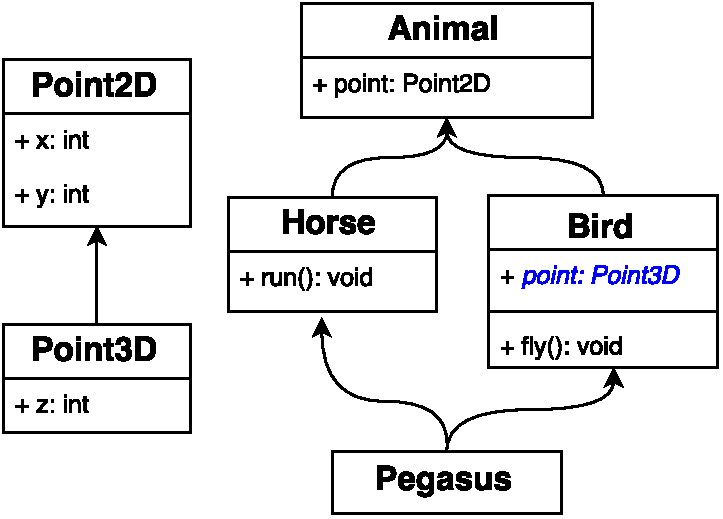
\includegraphics[height=3.8cm]{PegasusDetail.pdf}\hspace{20pt} &
\begin{minipage}{7cm}
\vspace{-90pt}
\lstinputlisting[linerange=6-15]{../UseMixinLombok/src/pegasusJava/Main.java}% APPLY:linerange=PEGASUS_JAVA
%basicstyle=\ttfamily\scriptsize
\end{minipage}
\end{tabular}
\caption{The animal system (left: complete structure, right: code for simplified animal system).}\label{fig:pegasus}
\end{figure}

This section illustrates how object interfaces, expressed using the \mixinAnn{} annotation, enables powerful
idioms using multiple inheritance in Java.
To propose a standard example for multiple inheritance, we show \Q@Animal@s with a two-dimensional \Q@Point2D@ representing their \Q@location@.
Some kinds of animals are \Q@Horse@s and \Q@Bird@s.
Birds can \Q@fly@, thus their locations need to be three-dimensional \Q@Point3D@s.
Finally, we model \Q@Pegasus@ (one of the best-known creatures in Greek
mythology) as a kind of \Q@Animal@ with the skills
of both \Q@Horse@s and \Q@Bird@s. A simple class diagram illustrating
the basic system is given in the left side of Figure~\ref{fig:pegasus}.\footnote{
Some research argues in favour of using subtyping for modelling taxonomies, other research argues against this practice, we do not wish to take sides in this argument, but to provide an engaging example.}

\subsection{Simple Multiple Inheritance with Default
  Methods}\label{sec:simple}

Before modelling the complete animal system, we  start with a
simplified version without locations. This version serves the purpose of illustrating how
Java 8 default methods can already model simple forms of multiple inheritance.
\texttt{Horse} and \texttt{Bird} are subtypes
of \texttt{Animal}, with methods \texttt{run()} and \texttt{fly()},
respectively. Pegasus can not only \emph{run} but also \emph{fly}! This is the
place where \emph{``multiple inheritance''} is needed, because
\texttt{Pegasus} needs to obtain \texttt{fly} and \texttt{run}
functionality from both \texttt{Horse} and \texttt{Bird}.
A first attempt to model the animal system in Java 8 is given on the right-side
of Figure~\ref{fig:pegasus}.
Note that the implementations of the methods \texttt{run}
and \texttt{fly} are defined inside interfaces, using default
methods. Moreover, because interfaces support multiple interface
inheritance, the interface for \texttt{Pegasus} can inherit behaviour
from both \texttt{Horse} and \texttt{Bird}. Although Java interfaces
do not allow instance fields, no form of state is needed so far to
model the animal system.

\paragraph{Instantiation}
To use \texttt{Horse}, \texttt{Bird} and \texttt{Pegasus}, some
objects must be created first. A first problem with using
interfaces to model the animal system is simply that interfaces
cannot be directly instantiated. Classes, such as:

\lstinputlisting[linerange=19-21]{../UseMixinLombok/src/pegasusJava/Main.java}% APPLY:linerange=PEGASUS_INST

\noindent are needed for instantiation. Now a \texttt{Pegasus} animal can be created
using the class constructor:

\begin{lstlisting}
Pegasus p = new PegasusImpl();
\end{lstlisting}

\noindent There are some annoyances here. Firstly, the sole
purpose of the classes is to provide a way to instantiate
objects. Although (in this case) it takes only one line of code to
provide each of those classes, this code is essentially boilerplate
code, which does not add behaviour to the system. Secondly,
the namespace gets filled with three additional types. For example,
both \texttt{Horse} and \texttt{HorseImpl} are needed: \texttt{Horse}
is needed because it needs to be an interface so that \texttt{Pegasus}
can use multiple inheritance; and \texttt{HorseImpl} is needed to
provide object instantiation.
Note that, for this very simple animal system, plain Java 8 anonymous
classes can be used to avoid these problems.  We could have simply
instantiated Pegasus using:

\begin{lstlisting}
Pegasus p = new Pegasus() {}; // anonymous class
\end{lstlisting}

\noindent However, as we shall see, once the system gets a little more
complicated, the code for instantiation quickly becomes more
complex and verbose (even with anonymous classes).

\subsection{Object Interfaces and Instantiation}

To model the animal system with object interfaces all that a user
needs to do is to add a \mixinAnn{} annotation to the \texttt{Horse},
\texttt{Bird}, and \texttt{Pegasus} interfaces:

\lstinputlisting[linerange=9-11]{../UseMixinLombok/src/pegasusLombok/Main.java}% APPLY:linerange=PEGASUS_LOMBOK

\noindent The effect of the annotations is that a static \emph{factory} method called
\texttt{of} is automatically added to the interfaces. With the
\texttt{of} method a Pegasus object is instantiated as follows:

\begin{lstlisting}
Pegasus p = Pegasus.of();
\end{lstlisting}

\noindent The \texttt{of} method provides an alternative to a
constructor, which is missing from interfaces. The following code,
shows the code corresponding to the \texttt{Pegasus} interface
after the \mixinAnn{} annotation is processed:

\begin{lstlisting}
interface Pegasus extends Horse, Bird { // generated code not visible to users
	static Pegasus of() {return new Pegasus() {};}}
\end{lstlisting}

\noindent Note that the generated code is transparent to a user, which
only sees the original code with the \mixin annotation. Compared to the pure
Java solution in Section~\ref{sec:simple}, the solution using object interfaces
has the advantage of providing a direct mechanism for object
instantiation, which avoids adding boilerplate classes to the
namespace.

\subsection{Object Interfaces with State}

The animal system modelled so far is a simplified version of the
system presented in the left-side of Figure~\ref{fig:pegasus}, which still does not appear to
justify the \mixinAnn{} annotation.  Now moving on to modelling
the complete animal system where \Q@Animal@s will include a \Q@location@
representing their position in space, we shall
see that modelling stateful components using plain Java 8 quickly becomes
cumbersome. The \mixinAnn{} annotation comes to rescue here and
allows avoiding significant amounts of boilerplate code.

\paragraph{\Q@Point2D@: simple immutable data with fields}
2D points should keep track of their coordinates.  The usual
approach to model points in Java would be to use a class with fields for the
coordinates. However here we will illustrate how points are modeled with
interfaces. Since Java disallows fields inside interfaces, state is modeled
using abstract (getter) methods:

\begin{lstlisting}
interface Point2D{ int x(); int y();}
\end{lstlisting}

\noindent Unfortunately, creating a new point object is cumbersome, even
with anonymous classes:

\begin{lstlisting}
Point2D p = new Point2D(){ public int x(){return 4;} public int y(){return 2;}}
\end{lstlisting}

\noindent However this cumbersome syntax is not required for every
object allocation. As programmers do, for ease or reuse, the boring
repetitive code can be encapsulated in a method. A generalization of the
\texttt{of} static factory method is appropriate in this case:
\begin{lstlisting}
interface Point2D{ int x(); int y();
  static Point2D of(int x, int y){return new Point2D(){
    public int x(){return x;} public int y(){return y;}};}}
\end{lstlisting}

\vspace{-5pt}
\paragraph{\Q@Point2D@ with Object Interfaces}
This obvious ``constructor'' code can be automatically generated by our \mixin
annotation.  By annotating the interface \Q@Point2D@, a variation of the shown
static method \texttt{of} will be generated, mimicking the functionality of a
simple-minded constructor. \mixin first looks at the abstract methods and detects
what are the fields, then generates an \Q@of@ method with one parameter for each
of them. That is, we can just write

\begin{lstlisting}
@Obj interface Point2D{ int x(); int y();}
\end{lstlisting}

\noindent More precisely, a field or factory parameter is generated for every
abstract method that takes no parameters (except for methods with special
names). An example of using \Q@Point2D@ is:
\begin{lstlisting}
Point2D p = Point2D.of(42,myPoint.y());
\end{lstlisting}
\noindent where we return a new point, using \Q@42@ as x-coordinate,
and taking all the other information (only \Q@y@ in this case) from
another point.

\paragraph{\texttt{wither} methods in Object Interfaces}
The pattern of creating a new object by reusing most information from an old
object is very common when programming with immutable
data-structures. As such, it is
supported in our code generation as \Q@with@ methods. For example:
\begin{lstlisting}
@Obj interface Point2D {
  int x();    int y(); // getters
  Point2D withX(int val);    Point2D withY(int val); /* with methods*/ }
\end{lstlisting}

\noindent Using \texttt{with} methods, the point \texttt{p} can be created instead using:

\begin{lstlisting}
Point2D p = myPoint.withX(42);
\end{lstlisting}

\noindent If there is a large number of fields, \texttt{with} methods
will save programmers from writing large amounts of tedious code that
simply copies field values.
\begin{comment}
is expanded by our annotation into\footnote{
Note how we actually generate a real field \Q@int x=_x;@.
This provides a more uniform translation that can work also for mutable data structures, where setters are required.
}

\begin{lstlisting}
interface Point2D{ int x(); int y();
  static Point2D of(int _x, int _y){return new Point2D(){
    int x=_x; int y=_y;
    public int x(){return x;}   public int y(){return y;}
    Point2D withX(int val){ return Point2D.of(val,this.y());}
    Point2D withY(int val){ return Point2D.of(this.x(),val);}
    };}
  Point2D withX(int val);    Point2D withY(int val);}
\end{lstlisting}
\end{comment}
Moreover, if the programmer wants a different implementation, he may
provide an alternative implementation using \Q@default@ methods. For example:
\begin{lstlisting}
@Obj interface Point2D{
  int x(); int y();
  default Point2D withX(int val){ ... };    default Point2D withY(int val){ ... }}
\end{lstlisting}

%\begin{comment}
%\marco{I re-enabled this code, I think is needed for understandability}
\noindent is expanded into
\begin{lstlisting}
interface Point2D{ int x(); int y();
  static Point2D of(int _x, int _y){return new Point2D(){
    int x=_x;    int y=_y;
    public int x(){return x;}    public int y(){return y;}
    };}
  default Point2D withX(int val){ ... }    default Point2D withY(int val){ ... }}
\end{lstlisting}

\noindent If an implementation is provided for methods,
only code for methods needing implementation is generated. Thus,
programmers can easily tailor the behaviour for their special needs.
%\end{comment}

%Firstly, to model \texttt{Point2D} that has x-coordinate and y-coordinate by an
%interface, we immediately run into the problem of expressing the fields
%\texttt{x} and \texttt{y}.
%interfaces. Method \texttt{withX, withY} creates a new instance of
%\texttt{Point2D} with updated field \texttt{x,y}, respectively.

% Firstly, to model \texttt{Animal} by an interface, we immediately run into the
% problem of expressing the field \texttt{point}. Since in Java there is no way to
% define member fields inside interfaces, we propose to simulate fields by
% abstract methods inside interfaces:

%\lstinputlisting[linerange=42-48]{../UseMixinLombok/src/test/TestAnimal.java}% APPLY:linerange=POINT2D

%\paragraph{Instantiation}
%In Java, to implement an interface like \texttt{Point2D}, a typical and trivial
%approach that programmers usually do is creating a class extending the interface
%and providing implementation for all methods inside. For example, this is the
%implementation for interface \texttt{Point2D}:

%\begin{lstlisting}
%class Point2DImpl implements Point2D {
%    private int _x;
%    private int _y;
%    public Point2DImpl(int x, int y) {
%        this._x = x;
%        this._y = y;
%    }
%    public int x() {
%        return _x;
%    }
%    public int y() {
%        return _y;
%    }
% %Your implementation of with is wrong
%    public Point2D withX(int x) {
%        x(x);
%        return this;
%    }
%    public void x(int x) {
%        _x = x;
%    }
%    public void y(int y) {
%        _y = y;
%    }
%    public Point2D withY(int y) {
%        y(y);
%        return this;
%    }
%}
%\end{lstlisting}
%
%\texttt{Point2DImpl} implements \texttt{Point2D} and provides a constructor with
%quite mechanical code. What's worse, the implementation in \texttt{Point2DImpl}
%may not be reused in a single inheritance language.

%
%\begin{lstlisting}
%  // inside interface Point2D
%  static Point of(int x, int y) {
%      return new Point() {
%          int _x = x;
%          int _y = y;
%          public int x() {
%            return _x;
%          }
%          public int y() {
%            return _y;
%          }
%          public Point2D withX(int x) {
%            x(x);
%            return this;
%          }
%          public void x(int x) {
%            _x = x;
%          }
%          public void y(int y) {
%            _y = y;
%          }
%          public Point2D withY(int y) {
%            y(y);
%            return this;
%          }
%    }
%  }
%\end{lstlisting}
%
%\lstinputlisting[linerange=15-27]{../UseMixinLombok/src/overview/TestPoint.java} % APPLY:linerange=POINT_OF

\paragraph{\Q@Animal@ and \Q@Horse@: simple mutable data with fields}
2D points are mathematical entities, thus we choose immutable data structure to
model them. However animals are real world entities, and when an animal moves,
it is the \emph{same} animal with a different location. We model this with
mutable state.

%Now we proceed to define \texttt{Animal} with \texttt{point} ``member
%field''.
%%Not again, before we used only getters!
% Again, we model this member field with getter and setter methods:
\lstinputlisting[linerange=58-58]{../UseMixinLombok/src/test/TestAnimal.java}% APPLY:linerange=ANIMAL

\noindent Here we declare abstract getter and setter for the mutable ``field''
\Q@location@.  Without the \mixin annotation, there is no convenient way to
instantiate \texttt{Animal}.  For \texttt{Horse}, the \mixin annotation is used
and an implementation of \texttt{run()} is defined using a \Q@default@
method. The implementation of \texttt{run()} further illustrates the convenience of \emph{with} methods:

\lstinputlisting[linerange=62-63]{../UseMixinLombok/src/test/TestAnimal.java}% APPLY:linerange=HORSE

\noindent Creating and using \texttt{Horse} is quite simple:

\lstinputlisting[linerange=10-12]{../UseMixinLombok/src/test/TestAnimal.java}% APPLY:linerange=USINGHORSE

\noindent Note how the \texttt{of}, \texttt{withX} and
\texttt{location} methods (all generated automatically) provide a
basic interface for dealing with animals.

\paragraph{Summary} Dealing with state (mutable or not) in object interfaces
relies on a notion of abstract state, where only methods that interact with
state are available to users. Object interfaces provide support for four
different types of abstract state operations, which are summarized in
Figure~\ref{fig:abstractstate}.  The abstract state operations are determined by
naming conventions and the types of the methods. Fluent setters are a variant of
conventional setters, and are discussed in detail in Section~\ref{sec:dsls}.

\begin{figure}
\begin{tabular}{|l|l|l|}
\hline
 & \textbf{Example}                  & \textbf{Description } \\ \hline
\textbf{``fields''/getters}        &   \Q@int x();@                  & Retrieves value from field \texttt{x}.          \\ \hline
{\bf withers}        &   \Q@Point2D withX(int val);@                & Clones
object; updates field \texttt{x} to \texttt{val}.             \\ \hline
\textbf{setters}        & \Q@void x(int val);@ & Sets the field
\texttt{x} to a  new value \texttt{val}.        \\ \hline
\textbf{fluent setters}        & \Q@Point2D x(int val);@ &Sets the field
\texttt{x} to \texttt{val} and returns \texttt{\this}.           \\ \hline
\end{tabular}

\caption{Abstract state operations, for a field \texttt{x}, allowed by the \mixin
  annotation. }

\label{fig:abstractstate}

\end{figure}

% by method
%\texttt{run()}: method \texttt{withX} returns a new point object with field
%\texttt{x} updated by the argument to \texttt{withX}. Without these
%\texttt{with} methods, operations like \texttt{run()} would be much harder to define.

\subsection{Object Interfaces and Subtyping}
\Q@Bird@s are \Q@Animal@s, but while \Q@Animal@s only need 2D
locations, \Q@Bird@s need 3D locations. Therefore when the \texttt{Bird}
interface extends the \Q@Animal@ interface, the notion of points needs to
be refined. Such kind of refinement usually poses a challenge
in typical class-based approaches. Fortunately, with object interfaces,
we are able to provide a simple and effective solution.

\paragraph{Unsatisfactory class-based solutions to field type refinement}
In Java if we define an animal class with a field we have a set of
unsatisfactory options in front of us:
\begin{itemize}
\item Define a \Q@Point3D@ field in \Q@Animal@: this is bad since all animals
  would require more than needed.
  %Also it requires the programmer to predict the future, or
  Also it requires adapting the old code to accommodate for new evolutions.

\item Define a \Q@Point2D@ field in \Q@Animal@ and define an extra \Q@int z@
  field in \Q@Bird@.  This solution is very ad-hoc, requiring to basically
  duplicate the difference between \Q@Point2D@ and \Q@Point3D@ inside \Q@Bird@.
  %Again, there are many reasons this would be bad,
  The most dramatic criticism is that it would not scale to a scenario when
  \Q@Bird@ and \Q@Point3D@ are from different programmers.

\item Redefine getters and setters in \Q@Bird@, always put \Q@Point3D@ objects
  in the field and cast the value out of the \Q@Point2D@ field to \Q@Point3D@
  when implementing the overridden getter.  This solution scales to the multiple
  programmers approach, but requires ugly casts and can be implemented in a
  wrong way leading to bugs.
\end{itemize}

We may be tempted to assume that a language extension is needed.
%Instead, with object interfaces, another approach is possible
Instead, the \emph{restriction} of (object) interfaces to have no
fields, enlighten us that another approach is possible; often in programming languages ``freedom is slavery''.

\paragraph{Field type refinement with object interfaces}
Object interfaces address the challenge of type-refinement as follows:
\begin{itemize}
\item by \emph{covariant method overriding} the return type of
  \texttt{location()} is refined to \texttt{Point3D};
\item by \emph{overloading} a new setter for location is defined with a more
  precise type;
\item a \Q@default@ setter implementation with the old signature is provided.
\end{itemize}

Thus, with object interfaces, the code for the \Q@Bird@ interface is:

\lstinputlisting[linerange=67-70]{../UseMixinLombok/src/test/TestAnimal.java}% APPLY:linerange=BIRD

%Interface \texttt{Point3D} extends \texttt{Point2D} with a new abstract method
%\texttt{int z()} (treated as a getter for member field \texttt{z}). Note that
%the return type of various methods (e.g. with- methods, getters) get refined
%either by covariant method overriding or automatically by our annotation
%processor. Besides \emph{with}, other methods (including \emph{clone},
%\emph{of}) also do type-refinements automatically.


\noindent From the type perspective, the key is the covariant method
overriding of \texttt{location()}. However, from the semantic
perspective the key is the implementation for the setter with the old
signature (\Q@location(Point2D)@). The key to the setter
implementation is a new type of \Q@with@ method, called a property updater.

\paragraph{\Q@Point3D@ and properties updaters}
The \Q@Point3D@ interface is defined as follows:

\lstinputlisting[linerange=52-55]{../UseMixinLombok/src/test/TestAnimal.java}% APPLY:linerange=POINT3D

\noindent \Q@Point3D@ includes a
\Q@with@ method, taking a \Q@Point2D@ as an argument.
Other wither methods (such as \Q@withX@) functionally update a field at a time.  This can be
inefficient, and sometimes hard to maintain.  Often we want to update multiple
fields simultaneously, for example using another object as source.  Following
this idea, the method \Q@with(Point2D)@ is an example of a (functional)
properties updater: it takes a certain type of object and returns a copy of the
current object with all fields that match the fields of updated
parameter type. The idea is that the result should be like \Q@this@, but
modified to be as similar as possible to the parameter.

With the new \Q@with@ method we may use the information for
\Q@z@ already stored in the object to forge an appropriate \Q@Point3D@
to store. Note how all the information about what fields sit in
\Q@Point3D@ and in \Q@Point2D@ is properly encapsulated in the
\Q@with@ method, and is transparent to the implementer of \Q@Bird@.

% To implement the old setter in a convenient way, \mixin supports one
% last type of operations: property updater \texttt{with}
% methods. Unlike the \texttt{withX} (where \texttt{X} stands for a
% field name) methods presented so far, property updaters take several
% fields at once, contained in an interface, and copy those fields into
% fields of another interface.



\begin{figure}
\lstinputlisting[linerange=79-91]{../UseMixinLombok/src/test/TestAnimal.java}% APPLY:linerange=GENERATED_POINT3D
\caption{Generated boilerplate code.}
\label{fig:boilerplate}
\end{figure}

\paragraph{Generated boilerplate}
Just to give a feeling on how much boring code \mixin is generating, we show the
generated code for the \texttt{Point3D} in Figure~\ref{fig:boilerplate}. The
generated code is mechanical. Writing such code by hand is error-prone. For
example a distracted programmer may swap the arguments of calls to
\Q@Point3D.of@.  Note how \Q@with-@ methods are automatically refined in their
return type, so that code like:

\begin{lstlisting}
Point3D p=Point3D.of(1,2,3); p=p.withX(42);
\end{lstlisting}

\noindent will be accepted. If the programmer wishes to suppress this behaviour
and keep the signature as it was, it is sufficient to redefine the \Q@with-@
methods in the new interface repeating the old signature.  Again, the philosophy
is that if the programmer provides something directly, \mixin does not touch it.
The cast in \Q@with(Point2D)@ is trivially safe because of the \Q@instanceof@
test. The idea is that if the parameter is a subtype of the current exact type,
then we can just return the parameter, as something that is just ``more'' than
\Q@this@.

\subsection{Advanced Multiple Inheritance with Object Interfaces}
Finally, defining \texttt{Pegasus} is as simple as we did in the simplified
(and stateless) version on the right-side of Figure~\ref{fig:pegasus}.
 Note how even the non-trivial pattern for field type refinement is
transparently composed, and \texttt{Pegasus} has a \Q@Point3D@
\Q@location@.%  This works because \Q@Horse@ do not perform
% any field type refinement, otherwise we may have to choose/create a
% common subtype in order for \texttt{Pegasus} to exists.

\lstinputlisting[linerange=74-74]{../UseMixinLombok/src/test/TestAnimal.java}% APPLY:linerange=PEGASUS


\begin{comment}
\subsection{A Running Example: \texttt{Point}}
Suppose we want to create a point component that models the a point in space,
that has x-coordinate and y-coordinate. For example, if we create the
\texttt{Point} interface in Java, it would look like this:

\begin{lstlisting}
interface Point {
    int x();
    int y();
}
\end{lstlisting}

\texttt{Point} has two (conceptually) member fields \texttt{x} and \texttt{y},
representing the two coordinates of a point. Methods \texttt{int x()} and
\texttt{int y()} serve as \emph{getter} methods.
% Methods \texttt{void X(int X)} and \texttt{void Y(int Y)} serve as
% \emph{setter} methods. Method \texttt{Point withX(int X)} updates field
% \texttt{X} and returns \textbf{this}.

\subsection{Naive Implementation}
In Java, to implement an interface like \texttt{Point}, a typical and trivial
approach that programmers usually do is creating a class extending the interface
and providing implementation for all methods inside. For example, this is the
implementation for interface \texttt{Point}:

\lstinputlisting[linerange=33-46]{../UseMixinLombok/src/overview/TestPoint.java} % APPLY:linerange=POINTIMPL

\texttt{PointImpl} implements \texttt{Point} and provides a constructor with
quite mechanical code. What's worse, the implementation in \texttt{PointImpl}
may not be reused in a single inheritance language.

\subsection{Our Approach}
Instead of writing a whole another class to provide the implementation for
\texttt{Point}, we annotate on interface \texttt{Point} directly with \mixin:

\lstinputlisting[linerange=6-10]{../UseMixinLombok/src/overview/TestPoint.java} % APPLY:linerange=POINT

The \mixin annotation will generate a static method \texttt{of} inside
\texttt{Point}. The method \texttt{of} mimic the functionality of constructors,
it takes arguments same as constructors and return objects similar to
constructors. It makes use of Java anonymous classes and achieves the same
implementation as \texttt{PointImpl}.

With our approach, we provide a Java annotation \mixin to provide default
implementations for various methods and a mechanism to instantiate
objects. \mixin annotation helps programmers to write less cumbersome code and
instantiate interfaces in Java.

\lstinputlisting[linerange=15-27]{../UseMixinLombok/src/overview/TestPoint.java} % APPLY:linerange=POINT_OF
\end{comment}


\begin{comment}
\subsection{More On \mixin}
Besides the benefit of freeing programmers from writing boilerplate code, our
\mixin annotation can also allow programs to mimic multiple inheritance in a
restricted form easily.

\lstinputlisting[linerange=42-48]{../UseMixinLombok/src/test/TestAnimal.java}% APPLY:linerange=POINT2D

\lstinputlisting[linerange=52-55]{../UseMixinLombok/src/test/TestAnimal.java}% APPLY:linerange=POINT3D

\lstinputlisting[linerange=58-58]{../UseMixinLombok/src/test/TestAnimal.java}% APPLY:linerange=ANIMAL

\lstinputlisting[linerange=62-63]{../UseMixinLombok/src/test/TestAnimal.java}% APPLY:linerange=HORSE

\lstinputlisting[linerange=67-70]{../UseMixinLombok/src/test/TestAnimal.java}% APPLY:linerange=BIRD

\lstinputlisting[linerange=74-74]{../UseMixinLombok/src/test/TestAnimal.java}% APPLY:linerange=PEGASUS

Interface \texttt{Point3D} extends \texttt{Point/Point2D} with a new abstract
method \texttt{int z()} (treated as a getter for member field
\texttt{z}). Interface \texttt{Horse} shows the usage and advantage of
\emph{with} methods by method \texttt{run()}: method \texttt{withX} returns a
new point object with field \texttt{x} updated by the argument to
\texttt{withX}. Without these \texttt{with} methods, operations like
\texttt{run()} would be much harder to define. Note that the return type of
various methods get refined automatically by our annotation processor. Besides
\emph{with}, other methods (including \emph{clone}, \emph{of}) also do
type-refinements automatically.

The \emph{``multiple inheritance''} case appears at interface
\texttt{Pegasus}. Pegasuses can not only \emph{run} but also \emph{fly}!
Interface \texttt{Pegasus} obtains \texttt{fly} and \texttt{run} functionality
through interface \texttt{Horse} and \texttt{Bird}. Using \mixin annotation,
actually these is no code at all programmers have to write. The idea of using
default methods inside interfaces was proposed in ~\cite{}. It enables us to do
multiple inheritance, which otherwise is hard to do in Java-like languages that
do not support multiple inheritance, easily.
\end{comment}
